% Ford-Fulkerson's bad example (generated by figs_c2ch06.py).
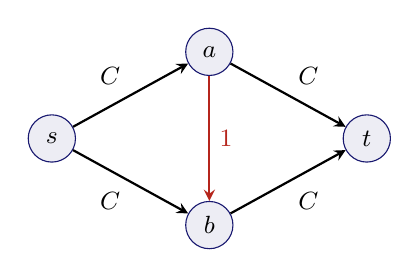
\begin{tikzpicture}[x=1cm,y=1cm,every node/.style={font=\small},>=stealth]
\tikzset{nd/.style={circle,draw=MidnightBlue,fill=MidnightBlue!8,inner sep=1pt,minimum size=0.6cm}}
\node[nd] (s) at (0,0) {$s$}; \node[nd] (a) at (2,1.1) {$a$}; \node[nd] (b) at (2,-1.1) {$b$}; \node[nd] (t) at (4,0) {$t$};
\draw[->,thick] (s) -- node[above left] {$C$} (a);
\draw[->,thick] (s) -- node[below left] {$C$} (b);
\draw[->,thick] (a) -- node[above right] {$C$} (t);
\draw[->,thick] (b) -- node[below right] {$C$} (t);
\draw[->,thick,BrickRed] (a) -- node[right] {$1$} (b);
\end{tikzpicture}
